\begin{figure*}
\raggedright
\begin{framed}
\begin{center}{\LARGE {\bf Model Card - Smiling Detection in Images}}\end{center} 
\vspace{1em}
    \begin{minipage}{.615\textwidth}
{\bf Model Details}
\begin{itemize}[leftmargin=*]
\item Developed by researchers at Google and the University of Toronto, 2018, v1.
\item Convolutional Neural Net.
\item Pretrained for face recognition then fine-tuned with cross-entropy loss for binary smiling classification.
\end{itemize}

\vspace{.25em}
{\bf Intended Use}
\begin{itemize}[leftmargin=*]
\item Intended to be used for fun applications, such as creating cartoon smiles on real images; augmentative applications, such as providing details for people who are blind; or assisting applications such as automatically finding smiling photos.
\item Particularly intended for younger audiences. 
\item Not suitable for emotion detection or determining affect; smiles were annotated based on physical appearance, and not underlying emotions.
\end{itemize}

\vspace{.25em}
{\bf Factors}
\begin{itemize}[leftmargin=*]
\item Based on known problems with computer vision face technology, potential relevant factors include groups for gender, age, race, and Fitzpatrick skin type; hardware factors of camera type and lens type; and environmental factors of lighting and humidity.
\item Evaluation factors are gender and age group, as annotated in the publicly available dataset CelebA \cite{LiuEtAl2015}.  Further possible factors not currently available in a public smiling dataset.  Gender and age determined by third-party annotators based on visual presentation, following a set of examples of male/female gender and young/old age.  Further details available in \cite{LiuEtAl2015}.
\end{itemize}

\vspace{.25em}
{\bf Metrics}
\begin{itemize}[leftmargin=*]
\item Evaluation metrics include {\bf False Positive Rate} and {\bf False Negative Rate} to measure disproportionate model performance errors across subgroups. {\bf False Discovery Rate} and {\bf False Omission Rate}, which measure the fraction of negative (not smiling) and positive (smiling) predictions that are incorrectly predicted to be positive and negative, respectively, are also reported. \cite{verma2018fairness}  
\item Together, these four metrics provide values for different errors that can be calculated from the confusion matrix for binary classification systems.
\item These also correspond to metrics in recent definitions of ``fairness'' in machine learning (cf. \cite{HardtEtAl2016,chouldechova2017fair}), where parity across subgroups for different metrics correspond to different fairness criteria.
\item 95\% confidence intervals calculated with bootstrap resampling.  
\item All metrics reported at the .5 decision threshold, where all error types (FPR, FNR, FDR, FOR) are within the same range (0.04 - 0.14). 
\end{itemize}
\vspace{.3em}
\begin{minipage}{0.4\textwidth}
{\bf Training Data}
\begin{itemize}[leftmargin=*]
\item CelebA \cite{LiuEtAl2015}, training data split. 
\end{itemize}
\vspace{1em}
\end{minipage}
\hspace{2em}
\begin{minipage}{0.5\textwidth}
    {\bf Evaluation Data}
\begin{itemize}[leftmargin=*]
\item CelebA \cite{LiuEtAl2015}, test data split.
\item Chosen as a basic proof-of-concept.
\end{itemize}
\end{minipage}

\vspace{-.25em}
{\bf Ethical Considerations}
\begin{itemize}[leftmargin=*]
\item Faces and annotations based on public figures (celebrities). No new information is inferred or annotated.
\end{itemize}
\end{minipage}
%\vspace{0.1em}
\begin{minipage}{0.31\textwidth}
\vspace{.5em}
{\bf Quantitative Analyses} \\%See Figure \ref{fig:smiling_error_rates_050}.
\begin{subfigure}{\textwidth}
\vspace{.25em}
\centering
\hbox{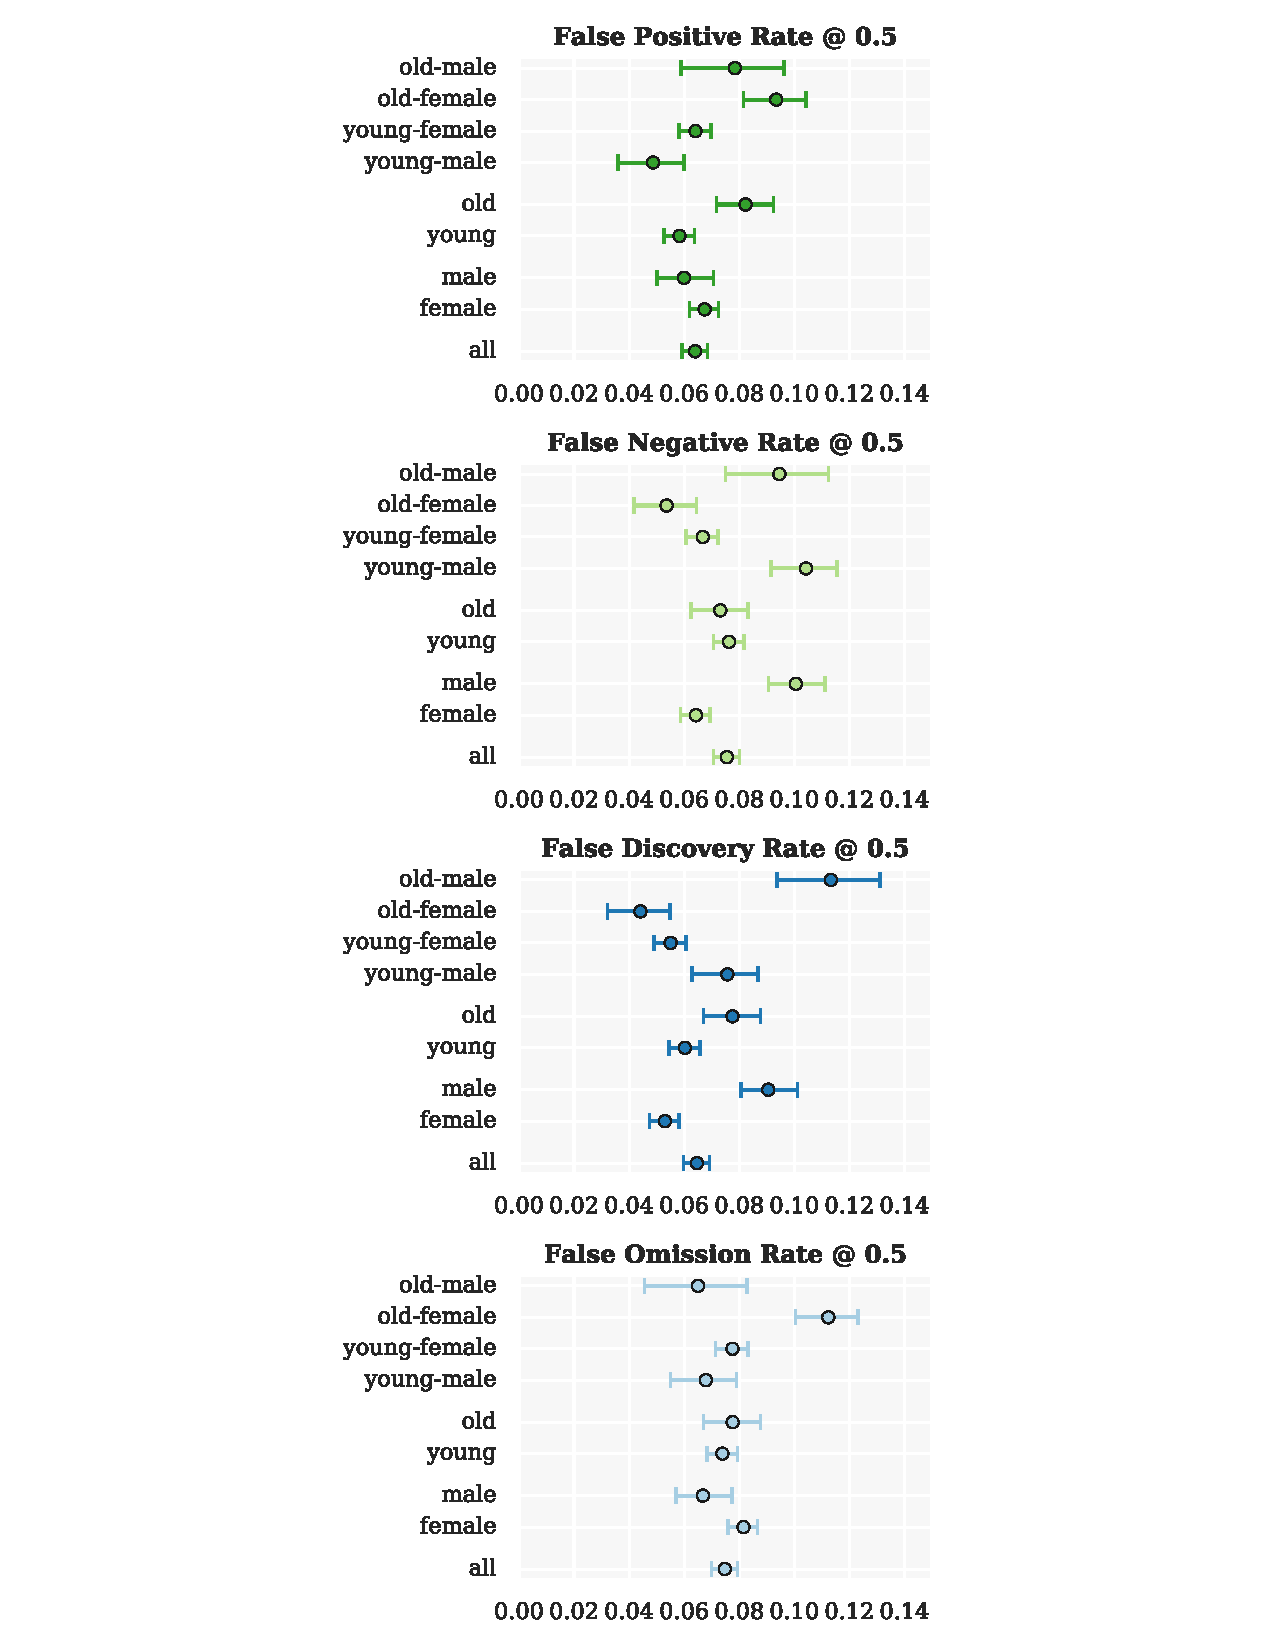
\includegraphics[scale=0.6,trim={5.1cm 0 0 0},clip]
{smiling_pointplots_spaced_exported.pdf}}
%\includegraphics[width=1\textwidth,height=0.7\textheight]
%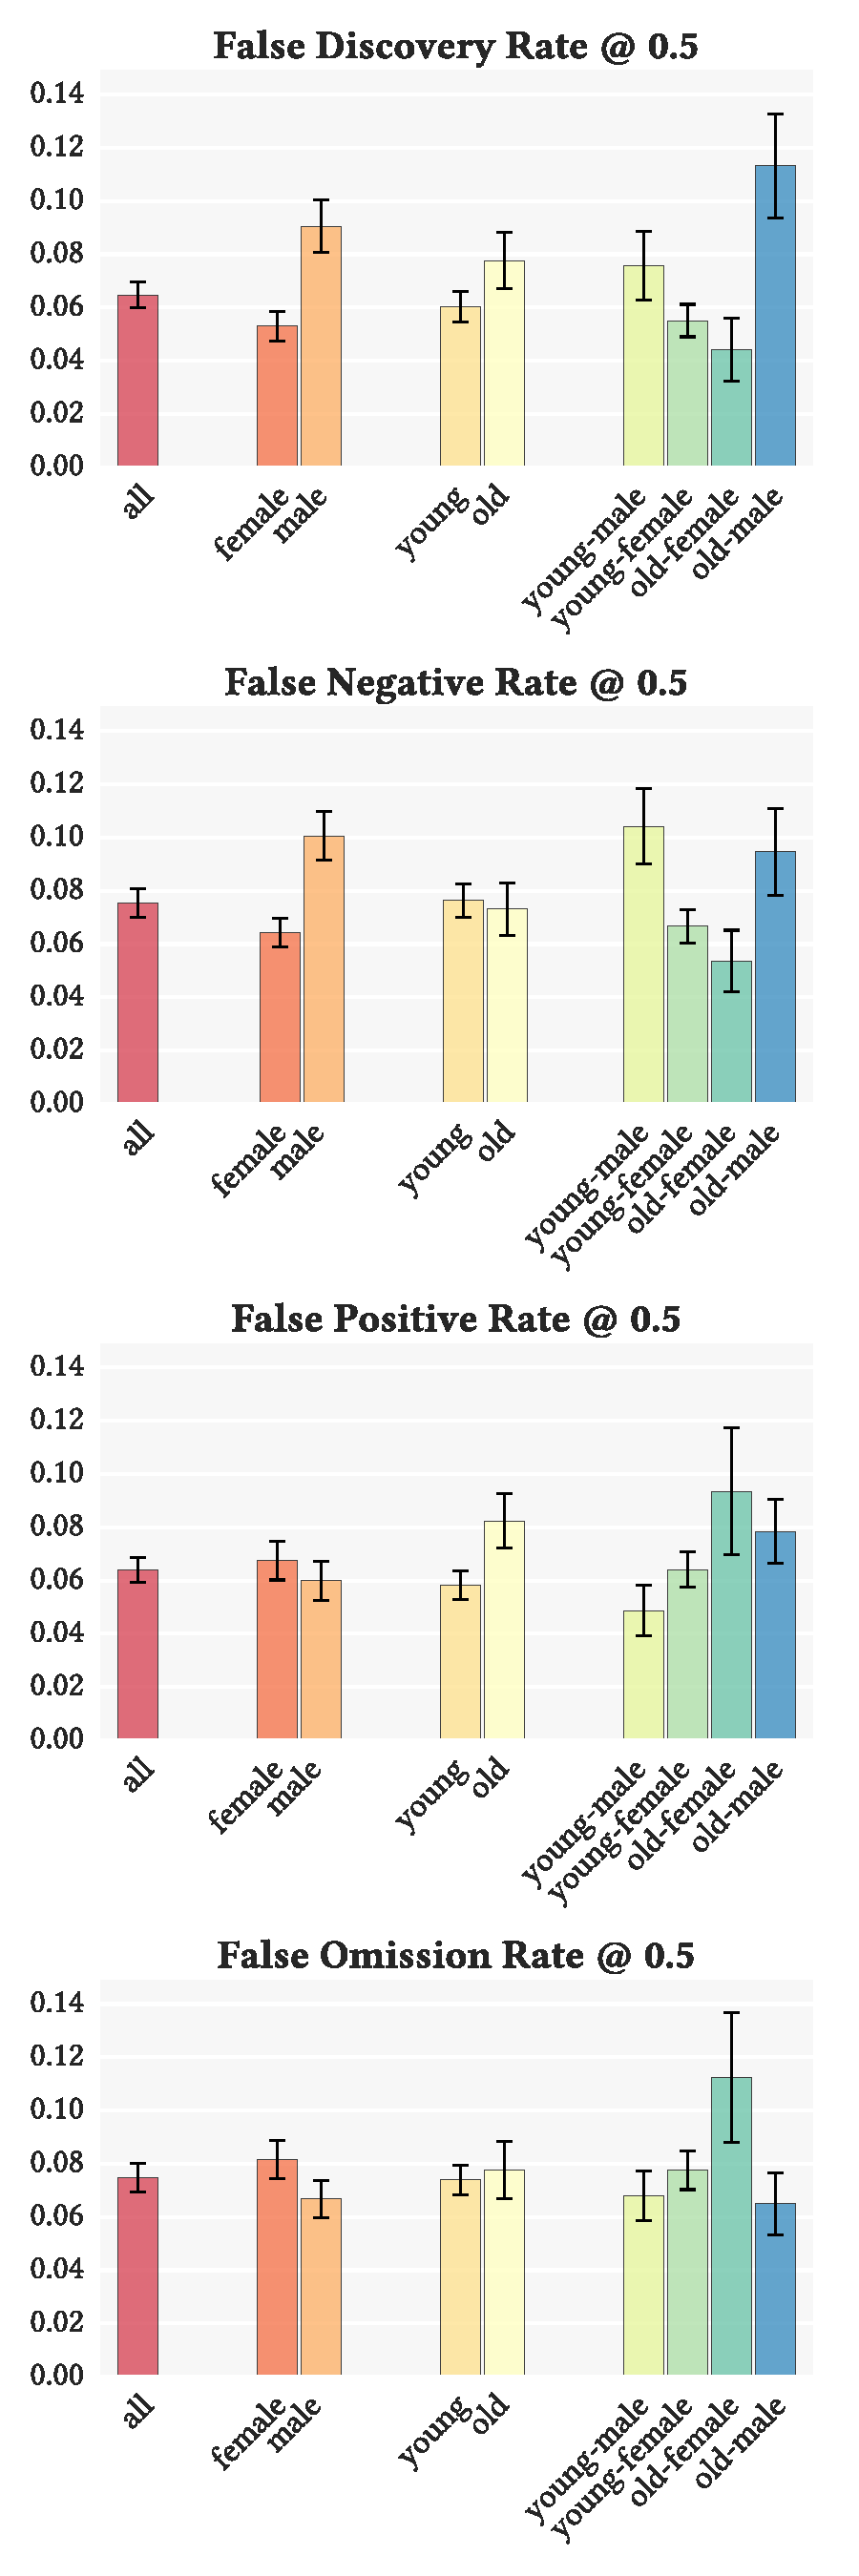
\includegraphics[width=1.2\textwidth]{smiling_error_rates_05.pdf}
\label{fig:celeba_error_rates_050}
\end{subfigure}
    \end{minipage}
\vspace{-.15em}    

{\bf Caveats and Recommendations}
\begin{itemize}[leftmargin=*]
\item Does not capture race or skin type, which has been reported as a source of disproportionate errors \cite{BuolamwiniGebru2018}.
\item Given gender classes are binary (male/not male), which we include as male/female. Further work needed to evaluate across a spectrum of genders.
\item An ideal evaluation dataset would additionally include annotations for Fitzpatrick skin type, camera details, and environment (lighting/humidity) details.
\end{itemize}    
\end{framed}
\vspace{-1em}
\caption{Example Model Card for a smile detector trained and evaluated on the CelebA dataset.}\label{fig:smiling_card}
\end{figure*}